
% ==========  Janelas deslizantes  ==========


%  Coesão léxica como presuposto básico
Os primeiros trabalhos dessa área se apoiam na ideia de que a mudança de assunto em um texto é acompanhada de uma proporcional mudança de vocabulário. Essa ideia, chamada de coesão léxica, sugere que a distribuição das palavras é um forte indicador da estrutura do texto, e demonstrou-se que há uma estreita correlação entre quedas na coesão léxica em janelas de texto e a transição de assuntos~\cite{Kozima1993}. Em seu trabalho, Kozima calculou a coesão léxica de uma janela de palavras usando \textit{spreading activation} em uma rede semântica especialmente elaborada para o idioma Inglês. Contudo, a implementação de um algoritmo para outros domínios depende da construção de uma rede adequada. 



O conceito de coesão léxica permite a aplicação da técnica de janelas deslizantes para encontrar os segmentos de um texto, em que se verifica a frequência dos termos em um fragmento do documento. Inicialmente, estabelece-se a partir do início do texto, um intervalo de $t$ termos, chamado janela que em seguida é deslocada em passos de $k$ termos adiante até o final do texto. A cada passo, analisa-se os termos contidos na janela.



% ==========  TextTiling  ==========

% Rafael --> Podem ter vários tipos de cursa. Ser mais objetivo. Quando a similaridade fica abaixo de um limiar fornecido pelo usuário.? Na verdade, dá pra fazer uma mescla. 

O conceito de coesão léxica motivou a elaboração dos primeiros algoritmos para segmentação textual, entre eles o \textit{TextTiling}. O \textit{TextTiling} baseia-se na ideia de que um segmento pode ser identificado pela análise dos termos que o compõe. Inicialmente, o \textit{TextTiling} recebe uma lista de candidatos a limite entre segmentos, usualmente finais de parágrafo ou finais de sentença. Utilizando a técnica de janelas deslizantes, para cada posição candidata são construídos 2 blocos, um contendo as sentenças que a precedem e outro com as que a sucedem. O tamanho desses blocos é um parâmetro a ser fornecido ao algoritmo e determina o tamanho mínimo de um segmento. Esse processo é ilustrado na Figura~\ref{fig:TT-slidingwindow}.



\begin{figure}[h!]
\center
	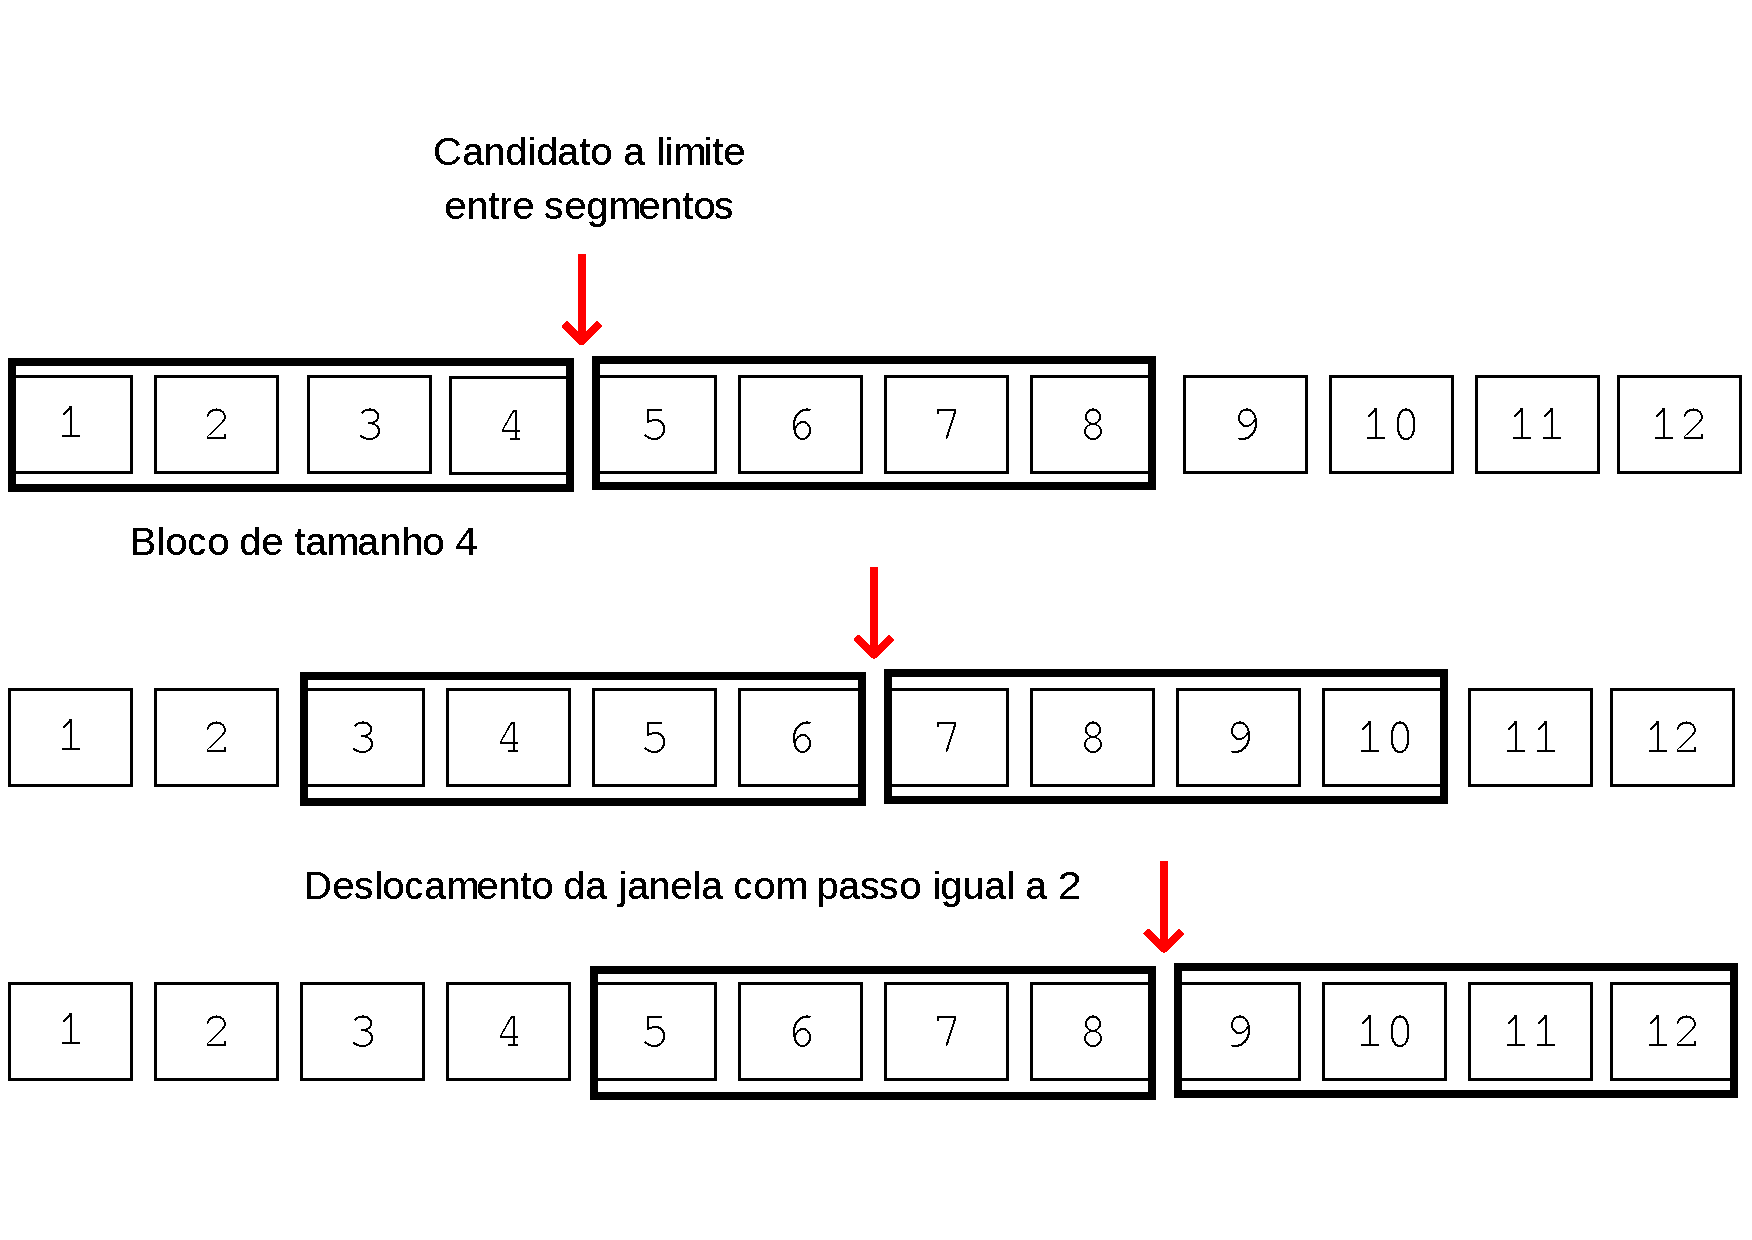
\includegraphics[trim={ 0 60 0 66 },clip,page=1,width=0.8\textwidth]{conteudo/capitulos/figs/janelas-deslizantes.pdf}

	\caption{Processo de deslocamento da janela deslizante. Os quadrados numerados representam as sentenças e os retângulos representam os blocos de texto a serem comparados. O deslocamento movimenta o candidato a limite e por consequência os blocos que o antecede e sucede.}
	\label{fig:TT-slidingwindow}
\end{figure}


Em seguida, os blocos de texto são representados por vetores que contém as frequências de suas palavras.  Diferente da proposta de Kozima, o \textit{TextTiling} utiliza cosseno (Equação~\ref{equ:cosine}) como medida para a similaridade entre os blocos adjacentes. Um limite ou transição entre segmentos é identificado sempre que a similaridade entre as unidades que antecedem e precedem o ponto candidato cai abaixo de um limiar, indicando uma diminuição da similaridade entre os blocos adjacentes. Ou seja, identifica-se uma transição entre segmentos pelos vales na curva de dissimilaridades. Para cada final de sentença representada por $c_i$ atribui-se uma profundidade dada por $(c_{i-1}-c_{i}) + (c_{i+1}-c_{i})$ e será um limite entre segmentos caso a profundidade exceda $\overline{s} - \sigma$, onde $\overline{s}$ é a média da profundidade de todos os vales do documento e $\sigma$, o desvio padrão. Na Figura~\ref{fig:curvasimilaridade} é ilustrado a curva de dissimilaridade entre os blocos adjacentes.  

   
\begin{figure}[h!]
\center
	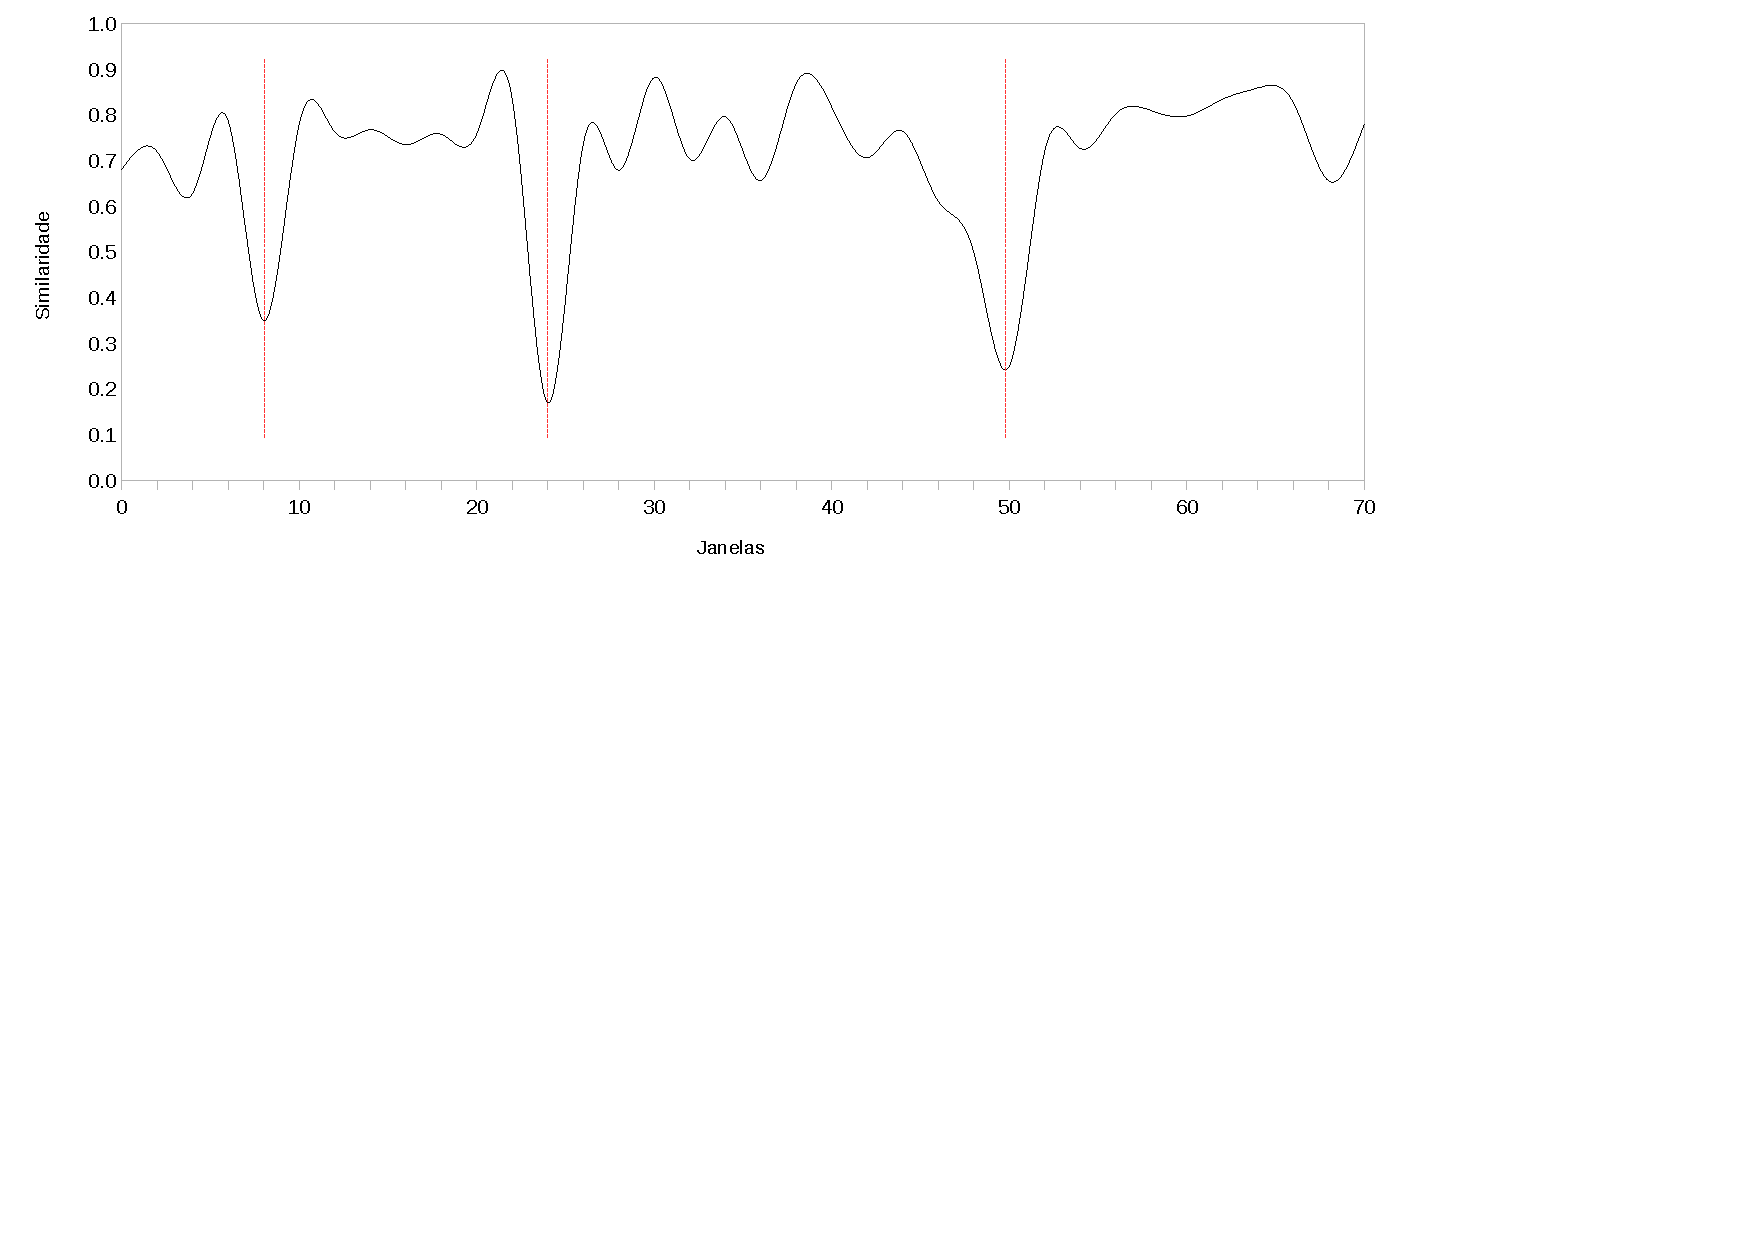
\includegraphics[trim={ 10 320 180 0 },clip,page=1,width=\textwidth]{conteudo/capitulos/figs/curva-similaridade.pdf}

	\caption{Curva de dissimilaridades entre blocos de texto adjacentes. As linhas pontilhadas representam diminuições de similaridade que indicam limites entre segmentos.}
	\label{fig:curvasimilaridade}
\end{figure}

% --> fazer um gráfico-rascunho e usar bolinhas para indicar os limites e usar 1 vale para demostrar o cálculo do depth score.


O TextTiling apresenta como vantagens a facilidade de implementação e baixa complexidade computacional, favorecendo a implementação de trabalhos similares ~\cite{Naili2016,Bokaei2015,CHAIBI2014,Kern2009,Galley2003}, e sua utilização como \texttit{base line} em outros trabalhos~\cite{Cardoso2017,Dias2007}. Por outro lado, algoritmos mais complexos, como os baseados em matrizes de similaridade, apresentam acurácia relativamente superior como apresentado em~\cite{Choi2000, Kern2009, Misra2009}.


% ==========  C99  ==========

Outro algoritmo frequentemente referenciado na literatura é o C99~\cite{Choi2000} o qual é baseado em uma matriz de \textit{ranking} das similaridades. A utilização de da coesão léxica pode não ser confiável para segmentos pequenos nessa abordagem, pois a ocorrência adicional de uma palavra pode causar certo impacto e alterar o cálculo da similaridade. Além disso, o estilo da escrita normalmente não é constante em todo o texto. Por exemplo, textos iniciais dedicados a introdução costumam apresentar menor coesão do que trechos dedicados a um tópico específico. Portanto, comparar a similaridade entre trechos de diferentes regiões não é apropriado. Devido a isso, as similaridades não podem ser comparadas em valores absolutos. Contorna-se esse problema fazendo uso de matrizes de similaridade para encontrar os segmentos de texto. Para isso, o \textit{C99} constrói uma matriz que contém as similaridades de todas as unidades de informação (normalmente sentenças ou parágrafos). 

%%%%%% 
%%%%%% 

Na Figura~\ref{fig:matrix-similarity} é mostrado um exemplo de uma matriz de similaridade onde a intensidade do ponto($i,j$) representa a similaridade entre as sentenças $i$ e $j$. Observa-se que a matriz é simétrica, assim cada ponto na linha diagonal representa a similaridade quando $i = j$ (ou seja, com a mesma sentença) e revela quadrados com maior concentração de pontos ao longo da diagonal. A concentração de pontos ao longo da diagonal indica porções de texto com maior coesão léxica.


  \begin{figure}[!h]
	  \centering
	  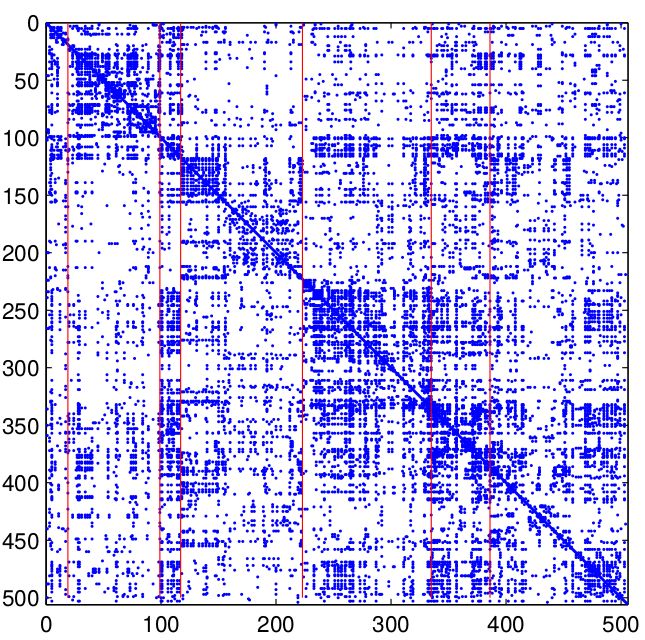
\includegraphics[width=0.6\textwidth]{conteudo/capitulos/figs/c99-ranking-matrix.png}
	  \caption{\textit{DotPlot} da similaridade entre sentenças onde as linha verticais representam segmentos reais~\cite{Eisenstein2008}.}
	  \label{fig:matrix-similarity}
  \end{figure}



%%%%%%%%%%%%%%%%%%%%%%%
% - Falar do esquema de ranking;
% - Imagem com os passos e máscara 3x3;
%%%%%%%%%%%%%%%%%%%%%%%

Em seguida, cada valor na matriz de similaridade é substituído por seu \textit{ranking} local. Para cada elemento da matriz, seu \textit{ranking} será o número de elementos vizinhos com valor de similaridade menor que o seu. Assim, para cada elemento determina-se uma região quadrada de tamanho $n$ em que o elemento em questão será comparado com $n \times n - 1$ elementos vizinhos.
% 
% 
Na Figura~\ref{fig:a} é destacado um quadro 3~x~3 de uma matriz. Tomando como exemplo o elemento com valor $0,5$, a mesma posição na matriz de \textit{rankings} terá o valor $4$, pois esse é o número de vizinhos com valores inferiores a $0,5$ dentro do quadro analisado na matriz de similaridades. Da mesma forma, na Figura~\ref{fig:b} para o valor $0,2$ a matriz de \textit{rankings} conterá o valor $1$ na mesma posição. Após a construção da matriz de ranking obtêm-se um maior contraste entre os pontos facilitando a detecção de limites quando a queda de similaridade entre sentenças é mais sutil.

\begin{figure}[!h]
	\centering     %%% not \center

	\subfigure[Passo 1]{\label{fig:a}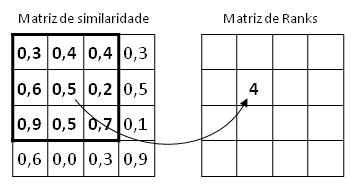
\includegraphics[width=60mm]{conteudo/capitulos/figs/exemplo-matrix-rank-A.png}
	\subfigure[Passo 2]{\label{fig:b}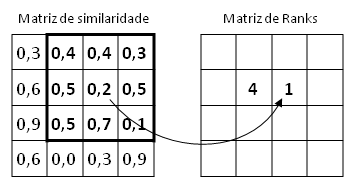
\includegraphics[width=60mm]{conteudo/capitulos/figs/exemplo-matrix-rank-B.png}
	
	\caption{Exemplo de construção de uma matriz de rankings.%~\cite{Choi2000}.
	}
	\label{fig:exemplomatrixrank}
\end{figure}
% -< Colocar uma explicação mais detalhada para esses passos




Finalmente, com base na matriz de \textit{ranking}, o C99 utiliza um método de \textit{clustering} baseado no algoritmo \textit{DotPloting}~\cite{Reynar1998} que usa regiões com maior densidade em uma matriz de similaridades para determinar como os segmentos estão distribuídos. Um segmento é definido por duas sentenças $i$ e $j$ que representam uma região quadrada ao longo da diagonal da matriz. Calcula-se a densidade dessa região como mostrado na Equação~\ref{equ:densidade-c99}. Seja $s_{i,j}$ a somatória dos \textit{rakings} de um segmento e $a_{i,j}$ sua área interior. Seja $B = \{b1,...,b_m\}$ a lista de $m$ segmentos e $s_k$ e $a_k$ são a somatória dos valores dos rankings e a área de um segmento $k$ em $B$. Então, a densidade é computada por: 

\begin{equation}
D = \frac{\sum_{k=1}^m s_k}{\sum_{k=1}^m a_k}
\label{equ:densidade-c99}
\end{equation}


O processo inicia com um único segmento formado por todas as sentenças do documento e o divide recursivamente em $m$ segmentos. Cada passo divide um dos segmentos em $B$ no ponto ($i,j$) que maximiza $D$~(Equação \ref{equ:densidade-c99}). O processo se repte até atingir o número de segmentos desejados ou um limiar de similaridade.
 


% ==========  TextSeg Utiyama and Isahara  ==========





% ==========  BayesSeg  ==========



Os métodos baseados em coesão léxica que utilizam métricas como cosseno quantificam a similaridade entre sentenças baseando-se apenas na frequência das palavras, Essa abordagem, ignora certas características do texto que podem dar pistas sobre a estrutura do texto. Por exemplo, frases como "Prosseguindo", "Dando continuidade", "Ao final da reunião" podem dar ajudar a detectar o inicio ou final de segmento. A fim de aproveitar esses indicadores, pode-se usar um framework bayesiano que permite incorporar fontes externas ao modelo. O método \textit{BayesSeg}~\cite{Eisenstein2008} aborda a coesão léxica em um contexto bayesiano onde as palavas de um segmento surgem de um modelo de linguagem multinomial o qual é associado a um assunto. 

Essa abordagem é similar à métodos probabilísticos de extração de tópicos como o Latent Dirichlet Allocation (LDA)~\cite{Blei2003}, com a diferença que ao invés de atribuir tópicos ocultos a cada palavra, esses são usados para segmentar o documento. Nesse sentido, detecta-se um limite entre sentenças quando a distribuição de tópicos entre elas for diferente.  O \textit{BayesSeg} baseia-se na ideia que alguns termos são usados em tópicos específicos enquanto outros são neutros em relação aos tópicos do documento e são usados para expressar uma estrutura do documento, ou seja, as "frases-pista" vem de um único modelo generativo. A fim de refletir essa ideia, o modelo é adaptado para influenciar a probabilidade da sentença de ser uma final ou início de segmento conforme a presença de "frases pista".


% ==========  MinCut  ==========

% file:///ext4Data/UFSCar/Dissertação-2018/referencias/Minimum Cut Model for Spoken Lecture Segmentation - article.pdf








